\documentclass[a4paper, 12pt]{extarticle}
\usepackage[top=1in, bottom=1in, left=1in, right=1in]{geometry}
\usepackage{amsmath}
\usepackage{amssymb}
\usepackage{graphicx}
\usepackage{hyperref}
\usepackage{tcolorbox}
\usepackage{tikz}
\usepackage{enumitem}
\usepackage{fontspec}
\usetikzlibrary{calc,decorations,patterns,arrows,decorations.pathmorphing,positioning,shapes}
\definecolor{pltblue}{HTML}{1F77B4}
\definecolor{pltgreen}{HTML}{2CA02C}
\definecolor{pltred}{HTML}{D62728}
\definecolor{pltorange}{HTML}{FF7F0E}
\tikzset{every picture/.style={/utils/exec={\fontspec{Humor Sans}}}}
\setmainfont{Pretty Neat}

\makeatletter
\pgfset{
  /pgf/decoration/randomness/.initial=2,
  /pgf/decoration/wavelength/.initial=100
}
\pgfdeclaredecoration{sketch}{init}{
  \state{init}[width=0pt,next state=draw,persistent precomputation={
    \pgfmathsetmacro\pgf@lib@dec@sketch@t0
  }]{}
  \state{draw}[width=\pgfdecorationsegmentlength,
  auto corner on length=\pgfdecorationsegmentlength,
  persistent precomputation={
    \pgfmathsetmacro\pgf@lib@dec@sketch@t{mod(\pgf@lib@dec@sketch@t+pow(\pgfkeysvalueof{/pgf/decoration/randomness},rand),\pgfkeysvalueof{/pgf/decoration/wavelength})}
  }]{
    \pgfmathparse{sin(2*\pgf@lib@dec@sketch@t*pi/\pgfkeysvalueof{/pgf/decoration/wavelength} r)}
    \pgfpathlineto{\pgfqpoint{\pgfdecorationsegmentlength}{\pgfmathresult\pgfdecorationsegmentamplitude}}
  }
  \state{final}{}
}
\tikzset{xkcd/.style={decorate,decoration={sketch,segment length=0.5pt,amplitude=0.5pt}}}
\makeatother

\usepackage{etoolbox}
\AtBeginEnvironment{tabular}{\fontspec{Humor Sans}}

\setlength{\parindent}{0pt}
\setlength{\parskip}{0.5em}
\usepackage{fancyhdr}
\usepackage{geometry}
\usepackage{adjustbox}
\usepackage{titling}
\date{}

\title{Building Your Code Time Machine\\{\large A Discovery Exercise}}
\author{}
\date{}

\begin{document}

\begin{center}
\Large\textbf{Building Your Code Time Machine}\\[0.5em]
\large A Discovery Exercise
\end{center}

\vspace{1em}

\noindent\textbf{The Problem}

You're working on a data analysis project. You have a file called \texttt{analysis.py}. Over the course of a week, you make many changes. Sometimes you break things. Sometimes you fix them. Sometimes you want to remember what you did yesterday.

This exercise will help you discover a system for tracking your work.

\section{Part 1: Saving Your Work}

\subsection{Your First Day}

You start with this code in \texttt{analysis.py}:

\begin{tcolorbox}[colback=white, colframe=black]
\begin{verbatim}
def calculate_mean(data):
    total = sum(data)
    return total / len(data)
\end{verbatim}
\end{tcolorbox}

\begin{enumerate}
    \item You realize this code crashes when \texttt{data} is empty. You fix it:

\begin{tcolorbox}[colback=white, colframe=black]
\begin{verbatim}
def calculate_mean(data):
    if len(data) == 0:
        return 0
    total = sum(data)
    return total / len(data)
\end{verbatim}
\end{tcolorbox}

Write down exactly what changed (use \texttt{+} prefix for lines added, \texttt{-} prefix for lines removed):

\vspace{3cm}

    \item Later that day, you add a new function:

\begin{tcolorbox}[colback=white, colframe=black]
\begin{verbatim}
def calculate_mean(data):
    if len(data) == 0:
        return 0
    total = sum(data)
    return total / len(data)

def calculate_median(data):
    sorted_data = sorted(data)
    return sorted_data[len(sorted_data) // 2]
\end{verbatim}
\end{tcolorbox}

Write down what changed this time (use \texttt{+} prefix for lines added, \texttt{-} prefix for lines removed):

\vspace{3cm}

\end{enumerate}

\subsection{Designing a Tracking System}

\begin{enumerate}[resume]
    \item You want to remember what your code looked like at different points in time. For each snapshot you save, what three pieces of information would be essential to include? Consider: How will you know when this snapshot was created? How will you remember what changes you made? How will you know what the code looked like at this point?

\vspace{4cm}

    \item You decide to save snapshots in boxes. Here's what you have so far:

\begin{center}
\begin{tcolorbox}[colback=pltblue!10, colframe=pltblue, width=0.8\textwidth, title=Snapshot 1]
\textbf{When:} Monday 9:00 AM\\
\textbf{Message:} "Started project"\\
\textbf{Files:} analysis.py (original version)
\end{tcolorbox}
\end{center}

\end{enumerate}

\subsection{Choosing What to Save}

You spend all morning working. You now have:
\begin{itemize}
    \item \texttt{analysis.py} (finished, working perfectly)
    \item \texttt{test.py} (finished, working perfectly)
    \item \texttt{scratch.py} (messy experimental code, not ready)
    \item \texttt{temp\_output.txt} (temporary file, you don't need it)
\end{itemize}

\begin{enumerate}[resume]
    \item You want to create a snapshot. Should you include all four files?

    \vspace{2cm}

    \item You realize you need a way to choose which files go into a snapshot. Design a system with three areas:

    \begin{center}
    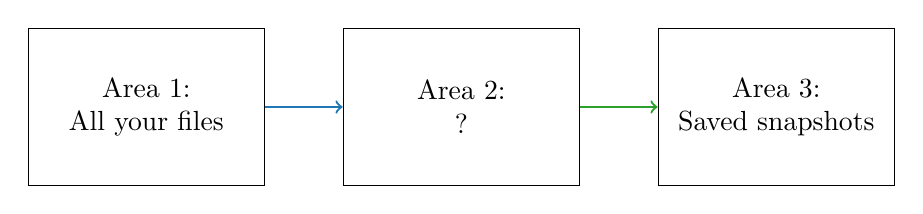
\begin{tikzpicture}[node distance=4cm]
        \node[draw, rectangle, minimum width=3cm, minimum height=2cm, align=center] (A) {Area 1:\\All your files};
        \node[draw, rectangle, minimum width=3cm, minimum height=2cm, align=center, right of=A] (B) {Area 2:\\?};
        \node[draw, rectangle, minimum width=3cm, minimum height=2cm, align=center, right of=B] (C) {Area 3:\\Saved snapshots};
        \draw[->, thick, pltblue] (A) -- (B);
        \draw[->, thick, pltgreen] (B) -- (C);
    \end{tikzpicture}
    \end{center}

    What should Area 2 be? What purpose does it serve? (Hint: Think about the problem you encountered with the four files earlier)

    \vspace{3cm}

    \item You have a file in Area 1 that you want to include in your next snapshot. What would you call the action of moving it to Area 2?

    \underline{\hspace{8cm}}

    You have files in Area 2 and you want to create a snapshot in Area 3 containing those files. What would you call this action?

    \underline{\hspace{8cm}}

    \vspace{1cm}

    \item Why is it useful to have Area 2 instead of going directly from Area 1 to Area 3?

    \vspace{3cm}

\end{enumerate}

\section{Part 2: Parallel Work}

\subsection{The Experiment Dilemma}

You want to try two completely different approaches to analyzing your data. You don't know which will work better. You want to try both without losing either one.

Your current snapshot history represents your stable, working code. This is the path that always works:

\begin{center}
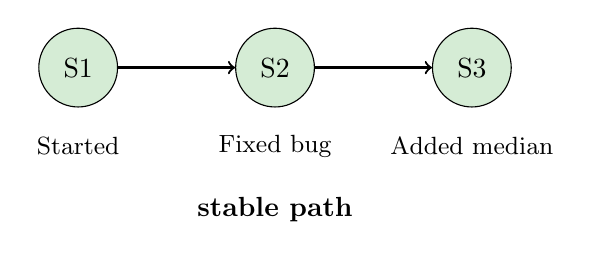
\begin{tikzpicture}[node distance=2.5cm]
    \node[draw, circle, fill=pltgreen!20, minimum size=1cm] (S1) {S1};
    \node[draw, circle, fill=pltgreen!20, minimum size=1cm, right of=S1] (S2) {S2};
    \node[draw, circle, fill=pltgreen!20, minimum size=1cm, right of=S2] (S3) {S3};
    \draw[->, thick] (S1) -- (S2);
    \draw[->, thick] (S2) -- (S3);
    \node[below of=S1, node distance=1cm] {\small Started};
    \node[below of=S2, node distance=1cm] {\small Fixed bug};
    \node[below of=S3, node distance=1cm] {\small Added median};
    \node[below of=S2, node distance=1.8cm] {\textbf{stable path}};
\end{tikzpicture}
\end{center}

\begin{enumerate}[resume]
    \item You want to try Method A and Method B starting from S3. Both will modify \texttt{analysis.py}. You want to keep the stable path stable and working. If you just keep making snapshots in a straight line on the stable path, what problem will you run into?

    \vspace{3cm}

    \item Starting from S3 on the stable path, you want to create snapshots for both Method A and Method B without losing either one or breaking the stable path. Draw what your snapshot history should look like. How can you arrange the snapshots so you can experiment with both methods while keeping the stable path stable?

    \vspace{5cm}

    \item You've created separate paths for experimentation while keeping the stable path stable. What would you call these experimental paths? Give them descriptive names based on what they're testing.

    \vspace{2cm}

\end{enumerate}

\section{Part 3: Hands-On with Git}

Now let's use actual Git commands to implement the system you designed. You'll create a repository, make commits, work with branches, and collaborate.

\subsection{Setup}

\textbf{Installing Git:}
\begin{itemize}
    \item \textbf{macOS:} Open Terminal and type \texttt{git --version}. If not installed, it will prompt you to install.
    \item \textbf{Windows:} Download from \url{https://git-scm.com/download/win} and install. Use Git Bash for commands.
\end{itemize}

\subsection{Exercise: Your First Repository}

Open your terminal (macOS) or Git Bash (Windows) and follow these steps:

\begin{enumerate}[resume]
    \item \textbf{Create a project folder and initialize Git:}

    \begin{tcolorbox}[colback=white, colframe=black]
    \begin{verbatim}
mkdir my-project
cd my-project
git init
    \end{verbatim}
    \end{tcolorbox}

    What did \texttt{git init} do? Check by running \texttt{ls -a} (macOS) or \texttt{dir /a} (Windows). You should see a \texttt{.git} folder.

    \vspace{2cm}

    \item \textbf{Create your first file and make a snapshot (commit):}

    \begin{tcolorbox}[colback=white, colframe=black]
    \begin{verbatim}
echo "print('Hello, Git!')" > hello.py
git add hello.py
git commit -m "Add hello script"
    \end{verbatim}
    \end{tcolorbox}

    Which part of your three-area system does \texttt{git add} implement? Which part does \texttt{git commit} implement?

    \vspace{2cm}

    \item \textbf{Create a branch for experiments:}

    \begin{tcolorbox}[colback=white, colframe=black]
    \begin{verbatim}
git branch experiment
git checkout experiment
echo "print('Experimental feature')" >> hello.py
git add hello.py
git commit -m "Add experimental feature"
    \end{verbatim}
    \end{tcolorbox}

    What does \texttt{git branch} do? What does \texttt{git checkout} do? How does this relate to the parallel paths you designed?

    \vspace{3cm}

    \item \textbf{Switch back to the main branch and check your file:}

    \begin{tcolorbox}[colback=white, colframe=black]
    \begin{verbatim}
git checkout main
cat hello.py
    \end{verbatim}
    \end{tcolorbox}

    (Use \texttt{type hello.py} instead of \texttt{cat} on Windows)

    What do you notice about the contents of \texttt{hello.py}? Why does it look different from when you were on the experiment branch?

    \vspace{3cm}

    \item \textbf{Merge your experiment into main:}

    \begin{tcolorbox}[colback=white, colframe=black]
    \begin{verbatim}
git merge experiment
cat hello.py
    \end{verbatim}
    \end{tcolorbox}

    What happened to \texttt{hello.py}? How does this relate to combining work from different paths?

    \vspace{3cm}

    \item \textbf{Setup remote repository (GitHub):}

    Create a free account at \url{https://github.com} if you don't have one. Then create a new repository called \texttt{my-project} (empty, no README).

    GitHub will show you commands. They'll look like this:

    \begin{tcolorbox}[colback=white, colframe=black]
    \begin{verbatim}
git remote add origin https://github.com/YOUR-USERNAME/my-project.git
git push -u origin main
    \end{verbatim}
    \end{tcolorbox}

    What does \texttt{git remote add} do? What does \texttt{git push} do? How does this relate to the backup server concept?

    \vspace{3cm}

    \item \textbf{Make a change on GitHub and pull it:}

    Go to your repository on GitHub. Click on \texttt{hello.py} and click the pencil icon to edit. Add a new line:

    \texttt{print("Edited on GitHub")}

    Click "Commit changes" at the bottom. Then in your terminal:

    \begin{tcolorbox}[colback=white, colframe=black]
    \begin{verbatim}
git pull
cat hello.py
    \end{verbatim}
    \end{tcolorbox}

    What does \texttt{git pull} do? How is this different from \texttt{git push}?

    \vspace{3cm}

\end{enumerate}

\section{Git}

The system you just designed and used is called \textbf{Git}. Here are the real names for the concepts you discovered:

\begin{tcolorbox}[colback=pltblue!10, colframe=pltblue]
\begin{itemize}
    \item \textbf{Snapshot} = Commit
    \item \textbf{Area 2 (choosing what to save)} = Staging Area
    \item \textbf{Parallel paths} = Branches
    \item \textbf{Combining work} = Merge
\end{itemize}
\end{tcolorbox}

\begin{enumerate}[resume]
    \item Now that you know the real names, write a short description of what Git is and why it's useful:

    \vspace{5cm}

\end{enumerate}

\end{document}
